\section{Paging: Smaller Tables}

%------------------------------------------------
\begin{frame}{The Problem: Page Tables Are Too Big}

\begin{itemize}
    \item 32-bit address space, 4KB pages, 4-byte PTE:
    \begin{itemize}
        \item $2^{32}/2^{12} \approx$ one million virtual pages;
        \item linear page table of \textbf{4MB} per process.
    \end{itemize}
    \item With a hundred active processes: hundreds of megabytes
          just for page tables!
\end{itemize}

\begin{block}{Crux: How to Make Page Tables Smaller?}
Simple array-based (linear) page tables are too big. How can we make page
tables smaller? What are the key ideas? What inefficiencies arise as a
result of these new data structures?
\end{block}

\end{frame}

%------------------------------------------------
\begin{frame}{Simple Solution: Bigger Pages}

\begin{itemize}
    \item 32-bit address space with \textbf{16KB pages}:
          18-bit VPN + 14-bit offset.
    \item $2^{18}$ entries $\times$ 4 bytes = \textbf{1MB} per page table
          (factor of four reduction).
    \item Problem: \textbf{internal fragmentation} (waste within each page).
    \item Most systems use small pages: 4KB (x86) or 8KB (SPARCv9).
\end{itemize}

\begin{block}{Aside: Multiple Page Sizes}
Many architectures (MIPS, SPARC, x86-64) support large pages (e.g., 4MB).
The main reason is not to save page-table space, but to
\textbf{reduce pressure on the TLB}. It makes the OS VM manager more complex.
\end{block}

\end{frame}

%------------------------------------------------
\begin{frame}{Most of a Linear Page Table Is Unused}

\begin{columns}[c]
    \begin{column}{0.50\textwidth}
        \begin{figure}
        \centering
        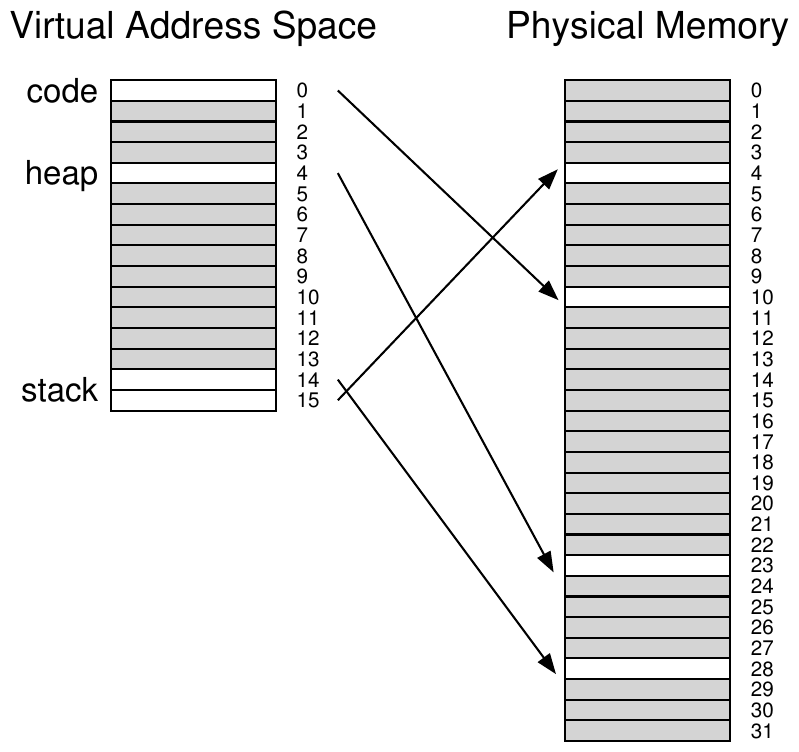
\includegraphics[height=0.55\textheight]{figs/chapter-20/figure-20.1.png}
        \caption*{Source: chapter page 3.}
        \label{fig:figure-20.1}
        \end{figure}
    \end{column}
    \begin{column}{0.46\textwidth}
        \begin{figure}
        \centering
        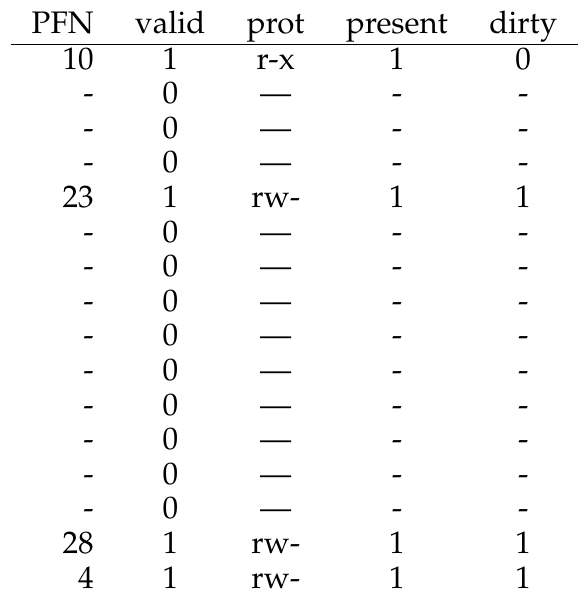
\includegraphics[height=0.45\textheight]{figs/chapter-20/figure-20.2.png}
        \caption*{Source: chapter page 3.}
        \label{fig:figure-20.2}
        \end{figure}
    \end{column}
\end{columns}

\begin{itemize}
    \item 16KB address space, 1KB pages: code (VPN 0), heap (VPN 4),
          stack (VPNs 14--15); the rest is \textbf{invalid}.
\end{itemize}

\end{frame}

%------------------------------------------------
\begin{frame}[fragile]{Hybrid Approach: Paging and Segments}

\begin{itemize}
    \item Idea from Multics (Jack Dennis): \textbf{one page table per
          logical segment} (code, heap, stack).
    \item MMU keeps base/bounds pairs per segment:
    \begin{itemize}
        \item \textbf{base}: physical address of the segment's page table;
        \item \textbf{bounds}: end of the page table (number of valid pages).
    \end{itemize}
    \item Top two bits of the virtual address select the segment:
\end{itemize}

\begin{center}
\renewcommand{\arraystretch}{1.3}
\begin{tabular}{|c|c|c|}
\hline
Seg (bits 31--30) & VPN (bits 29--12) & Offset (bits 11--0) \\
\hline
\end{tabular}
\end{center}

{\scriptsize
\begin{verbatim}
SN           = (VirtualAddress & SEG_MASK) >> SN_SHIFT
VPN          = (VirtualAddress & VPN_MASK) >> VPN_SHIFT
AddressOfPTE = Base[SN] + (VPN * sizeof(PTE))
\end{verbatim}
}

\end{frame}

%------------------------------------------------
\begin{frame}{Hybrid Approach: Pros and Cons}

\begin{itemize}
    \item Unallocated pages between stack and heap
          \textbf{no longer take up space} in a page table.
    \item But problems remain:
    \begin{itemize}
        \item still requires \textbf{segmentation}, which assumes a usage
              pattern; a large, sparsely-used heap still wastes page-table space;
        \item \textbf{external fragmentation} arises again: page tables now
              have arbitrary sizes (multiples of PTEs).
    \end{itemize}
\end{itemize}

\begin{block}{Tip: Use Hybrids}
When you have two good and seemingly opposing ideas, see if you can combine
them into a hybrid that achieves the best of both worlds.
\end{block}

\end{frame}

%------------------------------------------------
\begin{frame}{Multi-Level Page Tables}

\begin{columns}[T]

\column{0.40\textwidth}
\small
\begin{itemize}
    \item Turns the linear page table into something like a \textbf{tree}
          (used, e.g., by x86).
    \item Chop the page table into \textbf{page-sized units}; if a whole page
          of PTEs is invalid, \textbf{do not allocate it}.
    \item A new structure, the \textbf{page directory}, tracks where each page
          of the page table is (or that it holds no valid pages).
\end{itemize}

\column{0.58\textwidth}
\begin{figure}
    \centering
    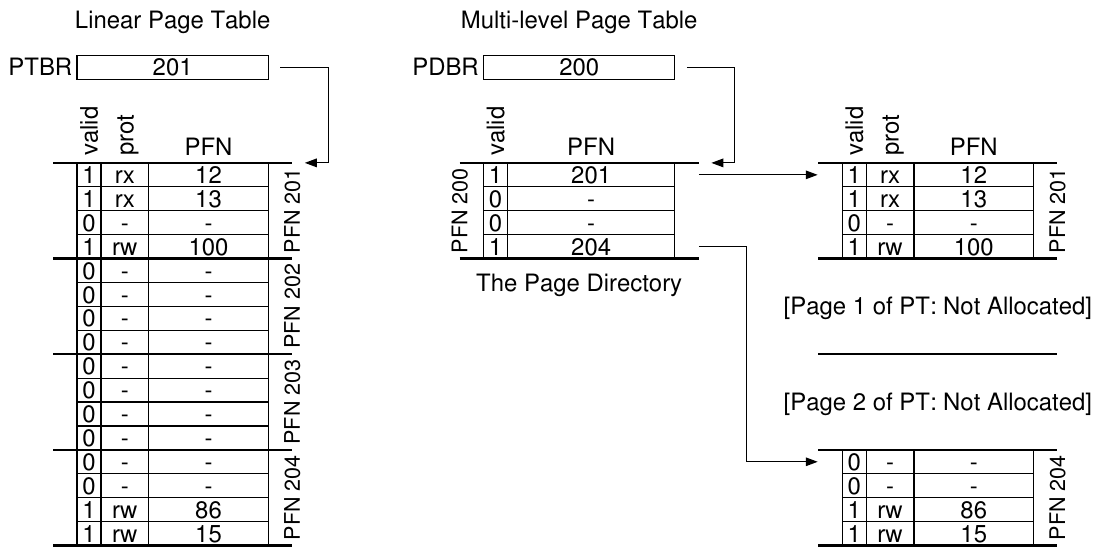
\includegraphics[width=1.0\linewidth]{figs/chapter-20/figure-20.3.png}
    \caption*{Source: chapter page 6.}
    \label{fig:figure-20.3}
\end{figure}

\end{columns}

\end{frame}

%------------------------------------------------
\begin{frame}{Page Directory Entries and Trade-offs}

\begin{itemize}
    \item \textbf{PDE}: valid bit + PFN; valid means at least one PTE in that
          page of the page table is valid.
    \item Advantages:
    \begin{itemize}
        \item space allocated in proportion to the address space in use
              (supports \textbf{sparse} address spaces);
        \item each piece fits in a page: page-table pages can be placed
              \textbf{anywhere} in physical memory.
    \end{itemize}
    \item Costs:
    \begin{itemize}
        \item on a TLB miss, \textbf{two loads} from memory
              (page directory + PTE);
        \item more \textbf{complexity} in the lookup.
    \end{itemize}
\end{itemize}

\begin{block}{Tip: Understand Time-Space Trade-offs}
Making a data structure faster usually costs space, and vice versa.
\end{block}

\end{frame}

%------------------------------------------------
\begin{frame}[fragile]{A Detailed Multi-Level Example}

\begin{columns}[T]

\column{0.62\textwidth}
\begin{itemize}
    \item 16KB address space, 64-byte pages: 14-bit address,
          8-bit VPN, 6-bit offset.
    \item Linear table: $2^8 = 256$ entries $\times$ 4 bytes = 1KB
          = \textbf{16 pages} of 16 PTEs each.
    \item Page directory: 16 entries, indexed by the
          \textbf{top 4 bits} of the VPN.
\end{itemize}

\begin{center}
\footnotesize
\renewcommand{\arraystretch}{1.3}
\begin{tabular}{|c|c|c|}
\hline
PDIndex (13--10) & PTIndex (9--6) & Offset (5--0) \\
\hline
\end{tabular}
\end{center}

{\tiny
\begin{verbatim}
PDEAddr = PageDirBase + (PDIndex * sizeof(PDE))
PTEAddr = (PDE.PFN << SHIFT) + (PTIndex * sizeof(PTE))
\end{verbatim}
}

\column{0.34\textwidth}
\begin{figure}
    \centering
    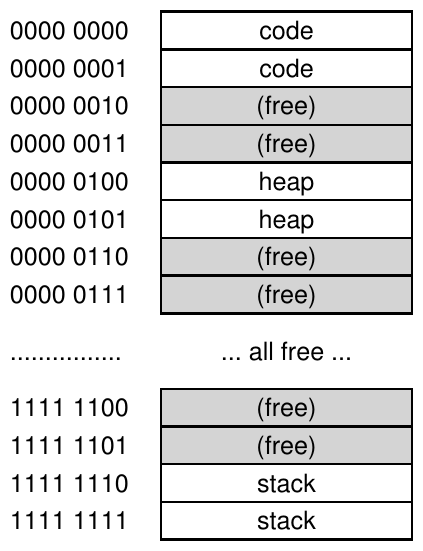
\includegraphics[height=0.55\textheight]{figs/chapter-20/figure-20.4.png}
    \caption*{Source: chapter page 8.}
    \label{fig:figure-20.4}
\end{figure}

\end{columns}

\end{frame}

%------------------------------------------------
\begin{frame}{Translating an Address}

\begin{columns}[T]

\column{0.42\textwidth}
\begin{itemize}
    \item Only \textbf{3 pages} allocated instead of 16:
          the directory + 2 pages of the page table.
    \item Address \texttt{0x3F80} = \texttt{11 1111 1000 0000}
          (byte 0 of VPN 254).
    \item PDIndex \texttt{1111} $\rightarrow$ PDE 15 $\rightarrow$ PFN 101.
    \item PTIndex \texttt{1110} $\rightarrow$ PTE 14 $\rightarrow$ PFN 55.
    \item PA $=$ \texttt{00 1101 1100 0000} $=$ \texttt{0x0DC0}.
\end{itemize}

\column{0.56\textwidth}
\begin{figure}
    \centering
    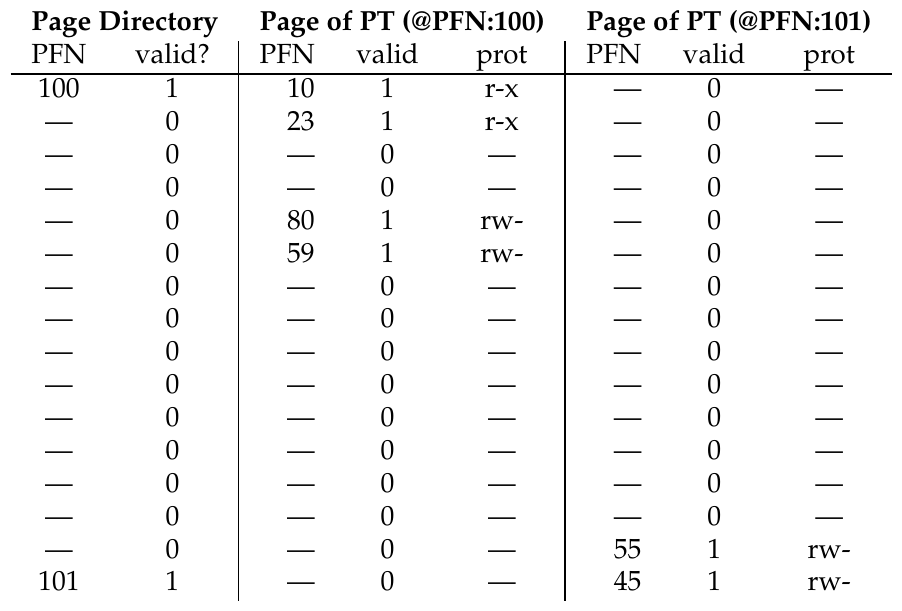
\includegraphics[width=1.0\linewidth]{figs/chapter-20/figure-20.5.png}
    \caption*{Source: chapter page 9.}
    \label{fig:figure-20.5}
\end{figure}

\end{columns}

\end{frame}

%------------------------------------------------
\begin{frame}{More Than Two Levels}

\begin{itemize}
    \item Goal: \textbf{every piece} of the multi-level table fits in a page.
    \item 30-bit address space, 512-byte pages: 21-bit VPN, 9-bit offset.
    \item 128 PTEs per page $\Rightarrow$ 7 bits of page-table index;
          the remaining 14 bits give a directory of $2^{14}$ entries
          spanning \textbf{128 pages}.
    \item Solution: split the page directory and add another level on top.
\end{itemize}

\begin{center}
\footnotesize
\renewcommand{\arraystretch}{1.3}
\begin{tabular}{|c|c|c|c|}
\hline
PD Index 0 & PD Index 1 & Page Table Index & Offset \\
\hline
\end{tabular}
\end{center}

\begin{block}{Tip: Be Wary of Complexity}
Implement the least complex system that achieves the task at hand.
\end{block}

\end{frame}

%------------------------------------------------
\begin{frame}{The Translation Process: Remember the TLB}

\begin{columns}[T]

\column{0.38\textwidth}
\begin{itemize}
    \item The TLB is checked \textbf{first}; on a hit, no page-table access.
    \item Only on a \textbf{TLB miss} is the full multi-level lookup done.
    \item Two-level table: \textbf{two additional memory accesses}
          per miss.
\end{itemize}

\column{0.60\textwidth}
\begin{figure}
    \centering
    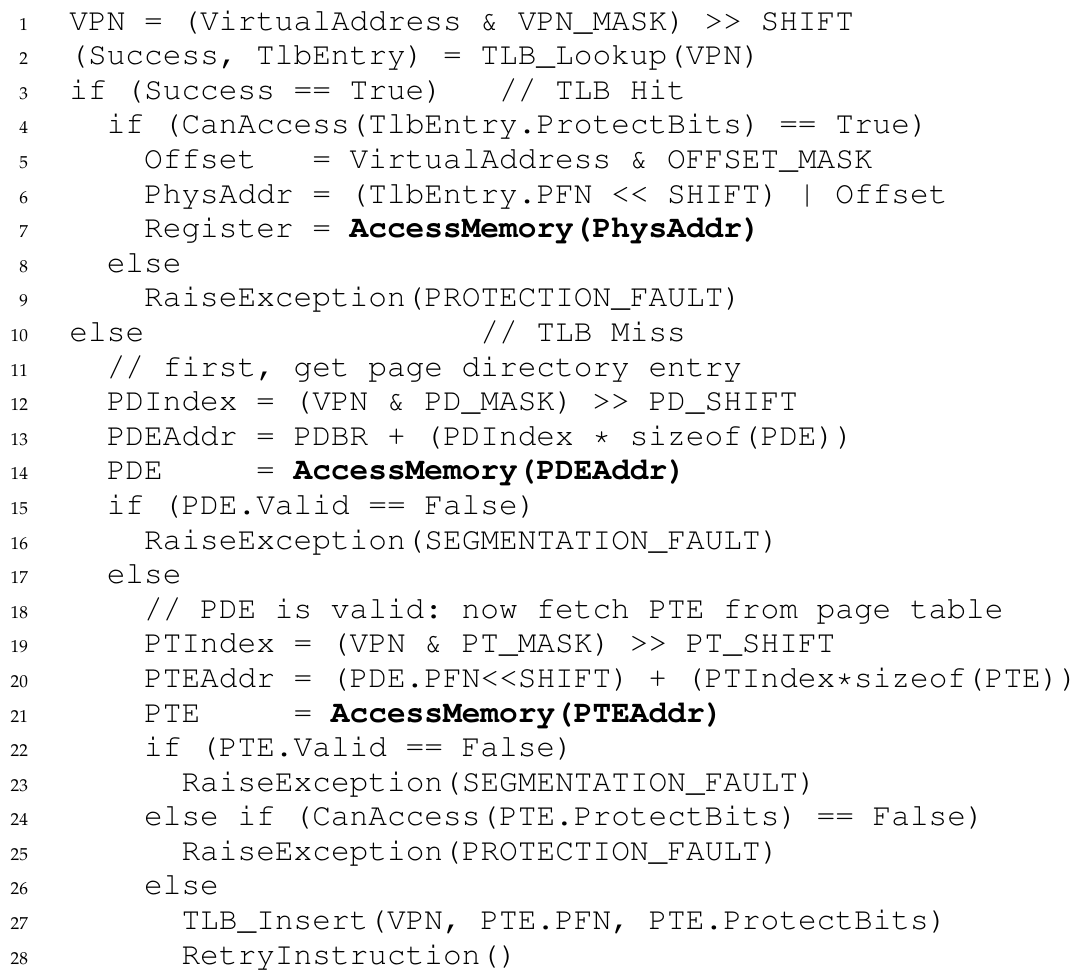
\includegraphics[height=0.68\textheight]{figs/chapter-20/figure-20.6.png}
    \caption*{Source: chapter page 12.}
    \label{fig:figure-20.6}
\end{figure}

\end{columns}

\end{frame}

%------------------------------------------------
\begin{frame}{Inverted Page Tables and Swapping}

\begin{itemize}
    \item \textbf{Inverted page table}:
    \begin{itemize}
        \item a \textbf{single} table with one entry per \textbf{physical page};
        \item each entry: which process and which virtual page use it;
        \item a \textbf{hash table} speeds up the search (e.g., PowerPC).
    \end{itemize}
    \item Page tables are \textbf{just data structures}.
    \item \textbf{Swapping page tables to disk}:
    \begin{itemize}
        \item some systems place page tables in \textbf{kernel virtual memory},
              allowing parts of them to be swapped out under memory pressure
              (more in the VAX/VMS case study).
    \end{itemize}
\end{itemize}

\end{frame}

%------------------------------------------------
\begin{frame}{Summary}

\begin{itemize}
    \item Real page tables are not necessarily linear arrays, but more
          complex data structures.
    \item Trade-off in \textbf{time and space}: the bigger the table,
          the faster a TLB miss can be serviced, and vice versa.
    \item Memory-constrained systems: small structures make sense.
    \item Plenty of memory and workloads using many pages:
          a bigger table that speeds up TLB misses may be better.
    \item Software-managed TLBs open the entire space of data structures
          to OS innovators.
\end{itemize}

\end{frame}

%------------------------------------------------
\begin{frame}{Homework (Simulation)}

\begin{itemize}
    \item Simulator: \texttt{paging-multilevel-translate.py}.
    \item How many registers are needed to locate a two-level page table?
          A three-level one?
    \item Translate addresses with random seeds 0, 1 and 2 (check with
          \texttt{-c}). How many memory references does each lookup need?
    \item How will memory references to the page table behave in the
          cache: many hits or many misses?
\end{itemize}

\end{frame}
